\begin{figure}[H]
\centering
\shorthandoff{<>}
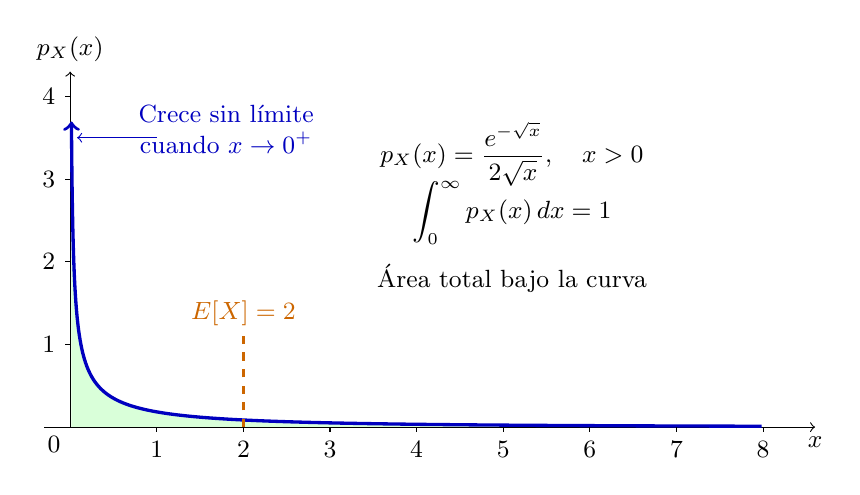
\begin{tikzpicture}[x=1.1cm,y=1.05cm,font=\small]
  \fill[green!15] (0.0144,0) --
    plot[domain=0.12:2.828427,samples=200,variable=\rootvalue]
    ({\rootvalue*\rootvalue},{exp(-\rootvalue)/(2*\rootvalue)})
    -- (8,0) -- cycle;
  \draw[->] (-0.3,0) -- (8.6,0) node[below] {$x$};
  \draw[->] (0,0) -- (0,4.3) node[above] {$p_X(x)$};
  \draw[blue!75!black,very thick,<-]
    plot[domain=0.12:2.828427,samples=200,variable=\rootvalue]
    ({\rootvalue*\rootvalue},{exp(-\rootvalue)/(2*\rootvalue)});
  \foreach \tick in {1,2,3,4,5,6,7,8}{
    \draw (\tick,0) -- (\tick,-0.06) node[below] {$\tick$};
  }
  \foreach \tick in {1,2,3,4}{
    \draw (0,\tick) -- (-0.06,\tick) node[left] {$\tick$};
  }
  \node[below left] at (0,0) {$0$};
  \draw[orange!80!black,dashed,thick] (2,0) -- (2,1.1)
    node[above] {$E[X]=2$};
  \node[align=center] at (5.1,3.3)
    {$\displaystyle p_X(x)=\frac{e^{-\sqrt{x}}}{2\sqrt{x}},\quad x>0$};
  \node[align=center] at (5.1,2.3)
    {$\displaystyle\int_0^\infty p_X(x)\,dx=1$\\[6pt]Área total bajo la curva};
  \node[align=center,text=blue!75!black] at (1.8,3.6)
    {Crece sin límite\\cuando $x\to0^+$};
  \draw[->,blue!75!black] (1,3.5) -- (0.08,3.5);
\end{tikzpicture}
\shorthandon{<>}

\smallskip
\(\displaystyle X=\frac{R-R_0}{\alpha h^2},\qquad
p_X(x)=\alpha h^2\,g(R_0+\alpha h^2x).\)
\caption{Densidad del radio efectivo en escala adimensional. La divergencia en el extremo izquierdo es integrable y no representa una probabilidad puntual en $R_0$. La curva continúa para $x>8$; su área total es uno. La línea discontinua señala la media $E[X]=2$, equivalente a $E[R]=R_0+2\alpha h^2$.}
\label{fig:densidad-radio}
\end{figure}